% 问题一·第二小问：质量冲突消解（正式章节）
% 由 sections/drafts/q1-conflict-results.tex 清洗接入：移除工作包元话语，统一图号与表述。
% 数据来源：run q1-conflict-*-2026092*（见 experiments/index.csv T-Q1-004）。
\subsubsection{第二小问：质量冲突消解}
\label{sec:q1-conflict}

\paragraph{从单一总分到多维冲突识别}
第一小问的 TOPSIS 总分对 16 个指标采取完全可补偿的聚合：一条“内容价值极高但广告含量高”的文本与一条“各维度均衡中等”的文本可能得到相同的总分。单一总分无法区分这两种结构不同的样本，而题目要求对“不同质量指标对同一文本给出显著不一致评价”的情形单独定义、消解。为此，本小问保留原总分 $Q_i^{(0)}$ 作为基线，回到多维信号层面识别冲突，再构造有限补偿的候选评分作为消解规则。冲突分析覆盖 $A_1$、$A_2$、$A_3$ 全部 $261{,}086$ 条唯一记录，沿用第一小问冻结的归一化与 CRITIC 权重（对原 TOPSIS 领域均分的复算误差小于 $10^{-12}$），并在扩展集上检验主要结论。

\paragraph{五维压缩与冲突定义}
将 16 个通用质量指标按语义压缩为五维，组内继承第一小问权重：
\begin{equation}
z_{ig}=\frac{\sum_{j\in G_g}w_jx_{ij}}{\sum_{j\in G_g}w_j},\qquad
v_g=\frac{\sum_{j\in G_g}w_j}{\sum_h\sum_{j\in G_h}w_j}.
\label{eq:q12-group}
\end{equation}
五维为内容价值、表达质量、整洁度、无广告程度和非重复程度。DSIR 三项与无字母词、句末标点的比例仍保留在原评分和对照试算中，不进入五维模型，该分组是适用性假设而非对这些指标有效性的否定。在 $A_1$ 拟合集上估计各维 $20\%$ 与 $80\%$ 分位数 $l_g=P_{20}(z_g)$、$h_g=P_{80}(z_g)$ 并冻结，定义
\begin{equation}
H_i=\{g:z_{ig}>h_g\},\quad L_i=\{g:z_{ig}<l_g\},\quad
I_i=\mathbf{1}\{H_i\neq\varnothing,\ L_i\neq\varnothing\}.
\label{eq:q12-conflict}
\end{equation}
$I_i=1$ 即判定为候选冲突样本：同一文本同时存在至少一个显著偏高维和至少一个显著偏低维。分位数给出的是相对于拟合分布的偏低或偏高的判断，不是语义缺陷真值，也不是统计显著性检验。按 $H_i$、$L_i$ 是否为空可将全部样本划分为四个互斥且穷尽的类别。进一步定义冲突强度与广度
\begin{equation}
C_i=\max_g\Big[\frac{z_{ig}-h_g}{1-h_g}\Big]_+ + \max_g\Big[\frac{l_g-z_{ig}}{l_g}\Big]_+,
\qquad
B_i=\frac{|H_i|\,|L_i|}{\binom{5}{2}},
\label{eq:q12-strength}
\end{equation}
其中 $[\,\cdot\,]_+$ 表示取正部；由于同一维度无法同时落入高低两端，故而 $C_i$ 的两项不是同一维。

\begin{table}[htbp]
  \centering
  \caption{五维阈值与组权重（由 $A_1$ 拟合集估计并冻结）}
  \label{tab:q1-conflict-thresholds}
  \renewcommand{\arraystretch}{1.15}
  \begin{tabular}{lrrr}
    \toprule
    维度 & 低阈值 & 高阈值 & 组权重 \\
    \midrule
    内容价值 & 0.2783 & 0.5613 & 0.2499 \\
    表达质量 & 0.3578 & 0.7702 & 0.2836 \\
    整洁度 & 0.2673 & 0.9884 & 0.1090 \\
    无广告程度 & 0.5244 & 0.9004 & 0.1056 \\
    非重复程度 & 0.6366 & 0.7838 & 0.2519 \\
    \bottomrule
  \end{tabular}
\end{table}

\paragraph{成因分析}
冲突的候选成因包括：同属性测量分歧（两种教育价值评分器一高一低，$A_1$ 中 415 条、全量去重中 1,402 条）、跨属性权衡（如教育产品推广可同时具有高内容价值与广告属性）、尺度与方向适用性（法律机构名称的必要复述可能触发重复性代理；非英语文本可能被英语流畅度拉低）、同源重复与领域构成变化。基于 15 个定向文本案例的机制分析只能说明存在候选机制，不能估计误判率或证明因果关系。分类器分歧与属性权衡可能存在重叠，不能直接相加计数。

\paragraph{有限补偿综合评价模型}
消解规则的设计目标是：对同属性测量分歧不武断地选择某个评分器，对跨属性权衡引入有界补偿。保留原评分 $Q_i^{(0)}$ 的同时，构造偏好权重的不确定集
\begin{equation}
\mathcal{W}_\lambda=\{(1-\lambda)v+\lambda p:\ p\ge0,\ \textstyle\sum_g p_g=1\},\qquad
Q_i^{\mathrm{cand}}=100\min_{a\in\mathcal{W}_\lambda}\sum_g a_gz_{ig}.
\label{eq:q12-robust}
\end{equation}
即以五维基线权重 $v$ 为中心、允许偏好向量在单纯形内偏离的最坏情形评分。令 $M_i=\sum_gv_gz_{ig}$、$m_i=\min_gz_{ig}$；线性目标在单纯形顶点处取得最小值，故式~\eqref{eq:q12-robust} 有闭式解
\begin{equation}
Q_i^{\mathrm{cand}}(\lambda)=100\big[(1-\lambda)M_i+\lambda m_i\big],\qquad
Q_i^{\mathrm{cand}}-100M_i=-100\lambda(M_i-m_i).
\label{eq:q12-closed}
\end{equation}
当 $0\le\lambda\le1$ 时，候选分位于 $[100m_i,\,100M_i]$ 内且对每一维取值不单调减；各维取值相同为 $c$ 时候选分恰为 $100c$。该规则连续作用于全部样本，不因离散冲突标签跨阈而产生突跳式扣分。$\lambda$ 刻画补偿的有界程度：$\lambda=0$ 退化为完全可补偿的加权均值，$\lambda=1$ 退化为五维最小值（完全不可补偿）。本文取 $\lambda=0.25$ 为主展示值，并比较 $\lambda\in\{0,0.1,0.25,0.5\}$ 的响应；在无外部效度证据前，不认定某一 $\lambda$ 是最优。

\paragraph{结果与扩展检验}
\begin{table}[htbp]
  \centering
  \caption{候选冲突的分层统计（阈值由 $A_1$ 拟合集冻结）}
  \label{tab:q1-conflict-coverage}
  \renewcommand{\arraystretch}{1.15}
  \begin{tabular}{lrrr}
    \toprule
    分区 & 样本数 & 候选冲突数 & 候选冲突率\% \\
    \midrule
    $A_1$ 全量 & 51,230 & 15,124 & 29.52 \\
    $A_1$ 留出 & 10,311 & 3,039 & 29.47 \\
    $A_2$ 重叠 & 1,419 & 798 & 56.24 \\
    $A_2$ 新增 & 16,104 & 9,408 & 58.42 \\
    $A_3$ 重叠 & 10,000 & 3,347 & 33.47 \\
    $A_3$ 新增 & 193,752 & 65,795 & 33.96 \\
    全量去重 & 261,086 & 90,327 & 34.60 \\
    \bottomrule
  \end{tabular}
\end{table}

$A_1$ 中四个类别样本数依次为 15,124、14,958、14,439、6,709，其中第一类即候选冲突类，占比 $29.52\%$，留出集为 $29.47\%$，一致性较好。分域看，arxiv 在 $A_1$ 中的候选冲突率为 $56.24\%$，其新增记录为 $58.42\%$；github 分别为 $33.47\%$ 与 $33.96\%$——两个唯一有新增记录的域上，扩展前后冲突水平接近，主要结论在扩展集上成立；其余五域没有扩展数据，构成不了独立验证。全量冲突率 $34.60\%$ 按 $A_1$ 领域比例重加权后为 $29.67\%$，总体增幅主要来自领域构成变化而非域内冲突水平变化。

\begin{figure}[htbp]
  \centering
  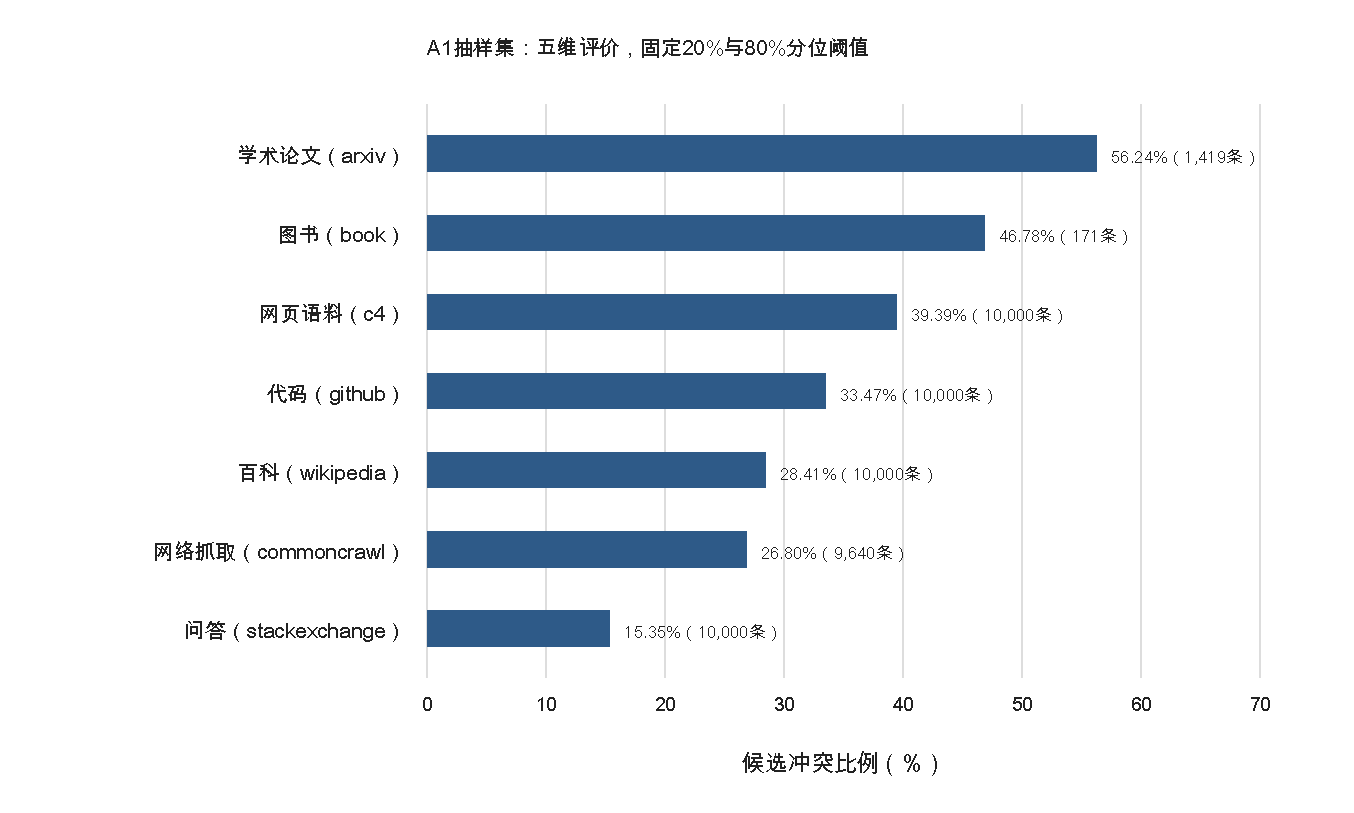
\includegraphics[width=.95\linewidth]{figures/fig1_domain_conflict.pdf}
  \caption{$A_1$ 七域候选冲突率及样本量，阈值由 $A_1$ 拟合集冻结。}
  \label{fig:q1-conflict-01}
\end{figure}

\begin{table}[htbp]
  \centering
  \caption{有限补偿候选评分（$\lambda=0.25$）}
  \label{tab:q1-conflict-resolution}
  \renewcommand{\arraystretch}{1.15}
  \begin{tabular}{lrrrr}
    \toprule
    分区 & 原TOPSIS均分 & 五维加权均分 & 候选稳健均分 & 相对五维基线变化 \\
    \midrule
    $A_1$ 全量 & 60.95 & 58.69 & 52.82 & -5.87 \\
    $A_1$ 留出 & 61.04 & 58.75 & 52.86 & -5.89 \\
    $A_2$ 新增 & 63.47 & 76.54 & 72.25 & -4.29 \\
    $A_3$ 新增 & 51.69 & 46.93 & 40.43 & -6.50 \\
    全量去重 & 54.23 & 51.07 & 44.83 & -6.24 \\
    \bottomrule
  \end{tabular}
\end{table}

需要说明，候选分与原 TOPSIS 分的差距同时混入了指标集合（16 维对 5 维）与聚合方式的变化，不能整体归因于补偿参数 $\lambda$；只有“候选分相对五维加权基线”的变化可以归因于 $\lambda$。以 arxiv 新增样本为例，候选分与原分的 Spearman 秩相关为 $0.611$，说明消解规则对排序有实质影响，选择 $\lambda$ 不是无关紧要的细节。得分降低这个变化本身并不意味着评分更准确，其效度主要依赖外部锚定检验（见第~\ref{sec:results} 节的验证清单）。

\begin{figure}[htbp]
  \centering
  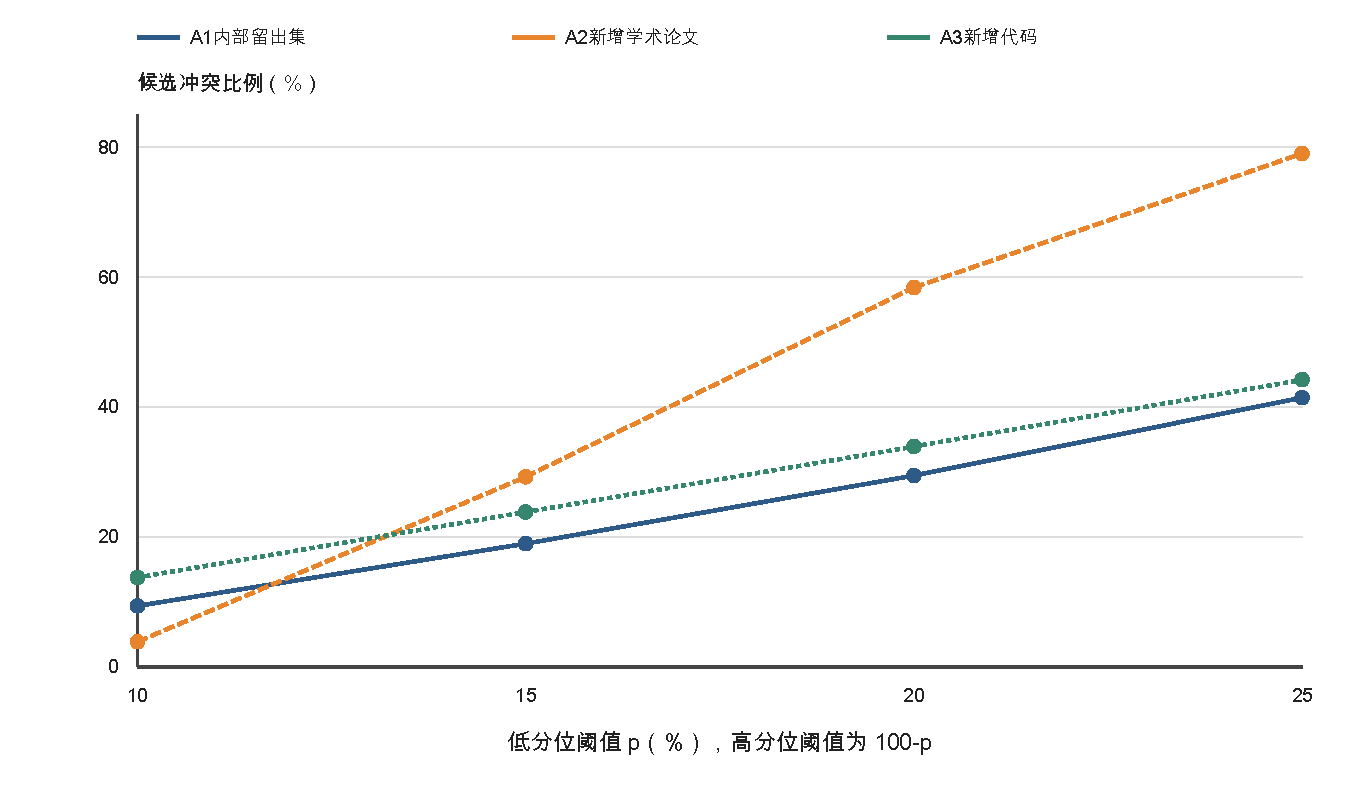
\includegraphics[width=.95\linewidth]{figures/fig2_threshold_sensitivity.pdf}
  \caption{冻结 $A_1$ 拟合参照下的阈值敏感性。}
  \label{fig:q1-conflict-02}
\end{figure}

\paragraph{阈值敏感性与适用边界}
冲突判定对阈值选择敏感：参照分位数由 P10/P90 改为 P25/P75 时，$A_1$ 冲突率由 $9.09\%$ 升至 $41.23\%$，arxiv 新增由 $3.89\%$ 升至 $79.07\%$，且域间相对排序改变。因此本文不以单一阈值的冲突率作为稳健结论，而将其作为随阈值单调响应的描述性量，主结果（扩展前后一致性、构成变化解释）在两种阈值下均成立。一个方向性的交叉检验支持阈值定义的合理性：按“高内容价值且相对低无广告”口径，$A_1$ 有 1,884 条；若改用更严格的“广告 logit 大于无广告 logit”原始口径则仅 310 条，说明相对分位口径捕捉的主要是轻度广告倾向而非强广告文本。

\begin{figure}[htbp]
  \centering
  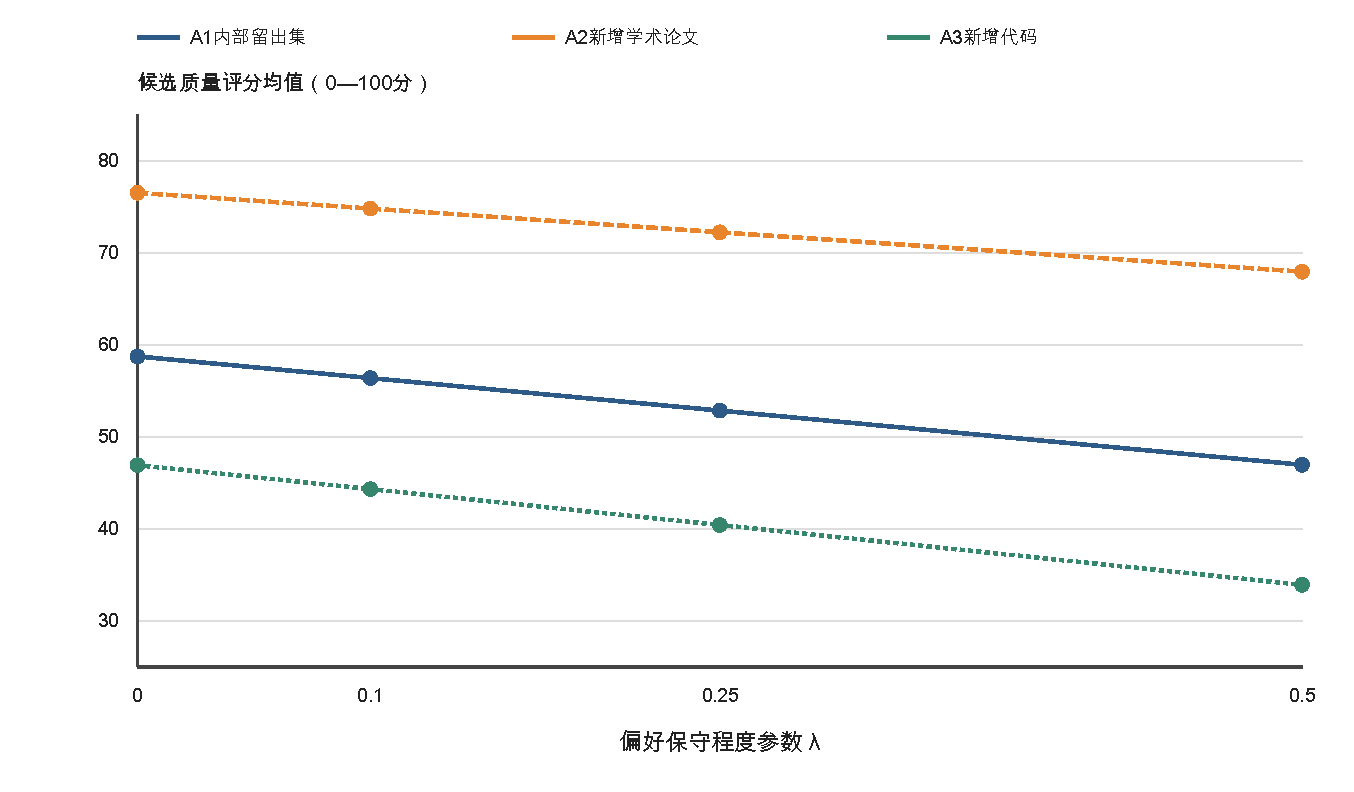
\includegraphics[width=.95\linewidth]{figures/fig3_compensation_sensitivity.pdf}
  \caption{补偿参数 $\lambda$ 对候选均分的影响。}
  \label{fig:q1-conflict-03}
\end{figure}

本小问的适用边界如下。第一，五维分组与冻结分位数均为建模选择，分组方案会主导冲突率水平，本文在固定分组下报告全部结果，分组稳健性分析列为后续工作。第二，目前无人工真值或下游 Loss 证据，候选消解规则的效度尚未外部锚定；据此构造的 83 条分层复核清单仍待标注，正式的 bootstrap 区间与权重扰动检验在本文版本中尚未执行。第三，冲突消解的输出是“带复核标记的候选评分”，不会自动替换第一小问的原评分；原评分继续作为后续三问的输入，候选评分用于敏感性分析。
